%% bare_conf.tex
%% V1.4a
%% 2014/09/17
%% by Michael Shell
%% See:
%% http://www.michaelshell.org/
%% for current contact information.
%%
%% This is a skeleton file demonstrating the use of IEEEtran.cls
%% (requires IEEEtran.cls version 1.8a or later) with an IEEE
%% conference paper.
%%
%% Support sites:
%% http://www.michaelshell.org/tex/ieeetran/
%% http://www.ctan.org/tex-archive/macros/latex/contrib/IEEEtran/
%% and
%% http://www.ieee.org/

%%*************************************************************************
%% Legal Notice:
%% This code is offered as-is without any warranty either expressed or
%% implied; without even the implied warranty of MERCHANTABILITY or
%% FITNESS FOR A PARTICULAR PURPOSE! 
%% User assumes all risk.
%% In no event shall IEEE or any contributor to this code be liable for
%% any damages or losses, including, but not limited to, incidental,
%% consequential, or any other damages, resulting from the use or misuse
%% of any information contained here.
%%
%% All comments are the opinions of their respective authors and are not
%% necessarily endorsed by the IEEE.
%%
%% This work is distributed under the LaTeX Project Public License (LPPL)
%% ( http://www.latex-project.org/ ) version 1.3, and may be freely used,
%% distributed and modified. A copy of the LPPL, version 1.3, is included
%% in the base LaTeX documentation of all distributions of LaTeX released
%% 2003/12/01 or later.
%% Retain all contribution notices and credits.
%% ** Modified files should be clearly indicated as such, including  **
%% ** renaming them and changing author support contact information. **
%%
%% File list of work: IEEEtran.cls, IEEEtran_HOWTO.pdf, bare_adv.tex,
%%                    bare_conf.tex, bare_jrnl.tex, bare_conf_compsoc.tex,
%%                    bare_jrnl_compsoc.tex, bare_jrnl_transmag.tex
%%*************************************************************************


% *** Authors should verify (and, if needed, correct) their LaTeX system  ***
% *** with the testflow diagnostic prior to trusting their LaTeX platform ***
% *** with production work. IEEE's font choices and paper sizes can       ***
% *** trigger bugs that do not appear when using other class files.       ***                          ***
% The testflow support page is at:
% http://www.michaelshell.org/tex/testflow/



\documentclass[conference]{IEEEtran}
% Some Computer Society conferences also require the compsoc mode option,
% but others use the standard conference format.
%
% If IEEEtran.cls has not been installed into the LaTeX system files,
% manually specify the path to it like:
% \documentclass[conference]{../sty/IEEEtran}





% Some very useful LaTeX packages include:
% (uncomment the ones you want to load)


% *** MISC UTILITY PACKAGES ***
%
%\usepackage{ifpdf}
% Heiko Oberdiek's ifpdf.sty is very useful if you need conditional
% compilation based on whether the output is pdf or dvi.
% usage:
% \ifpdf
%   % pdf code
% \else
%   % dvi code
% \fi
% The latest version of ifpdf.sty can be obtained from:
% http://www.ctan.org/tex-archive/macros/latex/contrib/oberdiek/
% Also, note that IEEEtran.cls V1.7 and later provides a builtin
% \ifCLASSINFOpdf conditional that works the same way.
% When switching from latex to pdflatex and vice-versa, the compiler may
% have to be run twice to clear warning/error messages.






% *** CITATION PACKAGES ***
%
%\usepackage{cite}
% cite.sty was written by Donald Arseneau
% V1.6 and later of IEEEtran pre-defines the format of the cite.sty package
% \cite{} output to follow that of IEEE. Loading the cite package will
% result in citation numbers being automatically sorted and properly
% "compressed/ranged". e.g., [1], [9], [2], [7], [5], [6] without using
% cite.sty will become [1], [2], [5]--[7], [9] using cite.sty. cite.sty's
% \cite will automatically add leading space, if needed. Use cite.sty's
% noadjust option (cite.sty V3.8 and later) if you want to turn this off
% such as if a citation ever needs to be enclosed in parenthesis.
% cite.sty is already installed on most LaTeX systems. Be sure and use
% version 5.0 (2009-03-20) and later if using hyperref.sty.
% The latest version can be obtained at:
% http://www.ctan.org/tex-archive/macros/latex/contrib/cite/
% The documentation is contained in the cite.sty file itself.


% \usepackage{graphicx}


% *** GRAPHICS RELATED PACKAGES ***
%
\ifCLASSINFOpdf
  \usepackage[pdftex]{graphicx}
  % declare the path(s) where your graphic files are
  \graphicspath{{.}}
  % and their extensions so you won't have to specify these with
  % every instance of \includegraphics
  \DeclareGraphicsExtensions{.pdf,.jpeg,.png,.jpg}
\else
  % or other class option (dvipsone, dvipdf, if not using dvips). graphicx
  % will default to the driver specified in the system graphics.cfg if no
  % driver is specified.
  % \usepackage[dvips]{graphicx}
  % declare the path(s) where your graphic files are
  % \graphicspath{{../eps/}}
  % and their extensions so you won't have to specify these with
  % every instance of \includegraphics
  % \DeclareGraphicsExtensions{.eps}
\fi
% graphicx was written by David Carlisle and Sebastian Rahtz. It is
% required if you want graphics, photos, etc. graphicx.sty is already
% installed on most LaTeX systems. The latest version and documentation
% can be obtained at: 
% http://www.ctan.org/tex-archive/macros/latex/required/graphics/
% Another good source of documentation is "Using Imported Graphics in
% LaTeX2e" by Keith Reckdahl which can be found at:
% http://www.ctan.org/tex-archive/info/epslatex/
%
% latex, and pdflatex in dvi mode, support graphics in encapsulated
% postscript (.eps) format. pdflatex in pdf mode supports graphics
% in .pdf, .jpeg, .png and .mps (metapost) formats. Users should ensure
% that all non-photo figures use a vector format (.eps, .pdf, .mps) and
% not a bitmapped formats (.jpeg, .png). IEEE frowns on bitmapped formats
% which can result in "jaggedy"/blurry rendering of lines and letters as
% well as large increases in file sizes.
%
% You can find documentation about the pdfTeX application at:
% http://www.tug.org/applications/pdftex





% *** MATH PACKAGES ***
%
%\usepackage[cmex10]{amsmath}
% A popular package from the American Mathematical Society that provides
% many useful and powerful commands for dealing with mathematics. If using
% it, be sure to load this package with the cmex10 option to ensure that
% only type 1 fonts will utilized at all point sizes. Without this option,
% it is possible that some math symbols, particularly those within
% footnotes, will be rendered in bitmap form which will result in a
% document that can not be IEEE Xplore compliant!
%
% Also, note that the amsmath package sets \interdisplaylinepenalty to 10000
% thus preventing page breaks from occurring within multiline equations. Use:
%\interdisplaylinepenalty=2500
% after loading amsmath to restore such page breaks as IEEEtran.cls normally
% does. amsmath.sty is already installed on most LaTeX systems. The latest
% version and documentation can be obtained at:
% http://www.ctan.org/tex-archive/macros/latex/required/amslatex/math/





% *** SPECIALIZED LIST PACKAGES ***
%
%\usepackage{algorithmic}
% algorithmic.sty was written by Peter Williams and Rogerio Brito.
% This package provides an algorithmic environment fo describing algorithms.
% You can use the algorithmic environment in-text or within a figure
% environment to provide for a floating algorithm. Do NOT use the algorithm
% floating environment provided by algorithm.sty (by the same authors) or
% algorithm2e.sty (by Christophe Fiorio) as IEEE does not use dedicated
% algorithm float types and packages that provide these will not provide
% correct IEEE style captions. The latest version and documentation of
% algorithmic.sty can be obtained at:
% http://www.ctan.org/tex-archive/macros/latex/contrib/algorithms/
% There is also a support site at:
% http://algorithms.berlios.de/index.html
% Also of interest may be the (relatively newer and more customizable)
% algorithmicx.sty package by Szasz Janos:
% http://www.ctan.org/tex-archive/macros/latex/contrib/algorithmicx/




% *** ALIGNMENT PACKAGES ***
%
%\usepackage{array}
% Frank Mittelbach's and David Carlisle's array.sty patches and improves
% the standard LaTeX2e array and tabular environments to provide better
% appearance and additional user controls. As the default LaTeX2e table
% generation code is lacking to the point of almost being broken with
% respect to the quality of the end results, all users are strongly
% advised to use an enhanced (at the very least that provided by array.sty)
% set of table tools. array.sty is already installed on most systems. The
% latest version and documentation can be obtained at:
% http://www.ctan.org/tex-archive/macros/latex/required/tools/


% IEEEtran contains the IEEEeqnarray family of commands that can be used to
% generate multiline equations as well as matrices, tables, etc., of high
% quality.




% *** SUBFIGURE PACKAGES ***
%\ifCLASSOPTIONcompsoc
%  \usepackage[caption=false,font=normalsize,labelfont=sf,textfont=sf]{subfig}
%\else
%  \usepackage[caption=false,font=footnotesize]{subfig}
%\fi
% subfig.sty, written by Steven Douglas Cochran, is the modern replacement
% for subfigure.sty, the latter of which is no longer maintained and is
% incompatible with some LaTeX packages including fixltx2e. However,
% subfig.sty requires and automatically loads Axel Sommerfeldt's caption.sty
% which will override IEEEtran.cls' handling of captions and this will result
% in non-IEEE style figure/table captions. To prevent this problem, be sure
% and invoke subfig.sty's "caption=false" package option (available since
% subfig.sty version 1.3, 2005/06/28) as this is will preserve IEEEtran.cls
% handling of captions.
% Note that the Computer Society format requires a larger sans serif font
% than the serif footnote size font used in traditional IEEE formatting
% and thus the need to invoke different subfig.sty package options depending
% on whether compsoc mode has been enabled.
%
% The latest version and documentation of subfig.sty can be obtained at:
% http://www.ctan.org/tex-archive/macros/latex/contrib/subfig/




% *** FLOAT PACKAGES ***
%
%\usepackage{fixltx2e}
% fixltx2e, the successor to the earlier fix2col.sty, was written by
% Frank Mittelbach and David Carlisle. This package corrects a few problems
% in the LaTeX2e kernel, the most notable of which is that in current
% LaTeX2e releases, the ordering of single and double column floats is not
% guaranteed to be preserved. Thus, an unpatched LaTeX2e can allow a
% single column figure to be placed prior to an earlier double column
% figure. The latest version and documentation can be found at:
% http://www.ctan.org/tex-archive/macros/latex/base/


%\usepackage{stfloats}
% stfloats.sty was written by Sigitas Tolusis. This package gives LaTeX2e
% the ability to do double column floats at the bottom of the page as well
% as the top. (e.g., "\begin{figure*}[!b]" is not normally possible in
% LaTeX2e). It also provides a command:
%\fnbelowfloat
% to enable the placement of footnotes below bottom floats (the standard
% LaTeX2e kernel puts them above bottom floats). This is an invasive package
% which rewrites many portions of the LaTeX2e float routines. It may not work
% with other packages that modify the LaTeX2e float routines. The latest
% version and documentation can be obtained at:
% http://www.ctan.org/tex-archive/macros/latex/contrib/sttools/
% Do not use the stfloats baselinefloat ability as IEEE does not allow
% \baselineskip to stretch. Authors submitting work to the IEEE should note
% that IEEE rarely uses double column equations and that authors should try
% to avoid such use. Do not be tempted to use the cuted.sty or midfloat.sty
% packages (also by Sigitas Tolusis) as IEEE does not format its papers in
% such ways.
% Do not attempt to use stfloats with fixltx2e as they are incompatible.
% Instead, use Morten Hogholm'a dblfloatfix which combines the features
% of both fixltx2e and stfloats:
%
% \usepackage{dblfloatfix}
% The latest version can be found at:
% http://www.ctan.org/tex-archive/macros/latex/contrib/dblfloatfix/




% *** PDF, URL AND HYPERLINK PACKAGES ***
%
%\usepackage{url}
% url.sty was written by Donald Arseneau. It provides better support for
% handling and breaking URLs. url.sty is already installed on most LaTeX
% systems. The latest version and documentation can be obtained at:
% http://www.ctan.org/tex-archive/macros/latex/contrib/url/
% Basically, \url{my_url_here}.




% *** Do not adjust lengths that control margins, column widths, etc. ***
% *** Do not use packages that alter fonts (such as pslatex).         ***
% There should be no need to do such things with IEEEtran.cls V1.6 and later.
% (Unless specifically asked to do so by the journal or conference you plan
% to submit to, of course. )


% correct bad hyphenation here
\hyphenation{op-tical net-works semi-conduc-tor}


\begin{document}
%
% paper title
% Titles are generally capitalized except for words such as a, an, and, as,
% at, but, by, for, in, nor, of, on, or, the, to and up, which are usually
% not capitalized unless they are the first or last word of the title.
% Linebreaks \\ can be used within to get better formatting as desired.
% Do not put math or special symbols in the title.
\title{Blockchain Based E-voting}


% author names and affiliations
% use a multiple column layout for up to three different
% affiliations
\author{\IEEEauthorblockN{Shane Lockwood}
\IEEEauthorblockA{Department of Computer Science\\
University of Colorado, Boulder\\
Boulder, Colorado 80309\\
Email: shane.lockwood@colorado.edu}
\and
\IEEEauthorblockN{Sham Prasad}
\IEEEauthorblockA{Department of Computer Science\\
University of Colorado, Boulder\\
Boulder, Colorado 80309\\
Email: shpa5747@colorado.edu}
\and
\IEEEauthorblockN{Ankur Jain}
\IEEEauthorblockA{Department of Computer Science\\
University of Colorado, Boulder\\
Boulder, Colorado 80309\\
Email: anja1834@colorado.edu}}

% conference papers do not typically use \thanks and this command
% is locked out in conference mode. If really needed, such as for
% the acknowledgment of grants, issue a \IEEEoverridecommandlockouts
% after \documentclass

% for over three affiliations, or if they all won't fit within the width
% of the page, use this alternative format:
% 
%\author{\IEEEauthorblockN{Michael Shell\IEEEauthorrefmark{1},
%Homer Simpson\IEEEauthorrefmark{2},
%James Kirk\IEEEauthorrefmark{3}, 
%Montgomery Scott\IEEEauthorrefmark{3} and
%Eldon Tyrell\IEEEauthorrefmark{4}}
%\IEEEauthorblockA{\IEEEauthorrefmark{1}School of Electrical and Computer Engineering\\
%Georgia Institute of Technology,
%Atlanta, Georgia 30332--0250\\ Email: see http://www.michaelshell.org/contact.html}
%\IEEEauthorblockA{\IEEEauthorrefmark{2}Twentieth Century Fox, Springfield, USA\\
%Email: homer@thesimpsons.com}
%\IEEEauthorblockA{\IEEEauthorrefmark{3}Starfleet Academy, San Francisco, California 96678-2391\\
%Telephone: (800) 555--1212, Fax: (888) 555--1212}
%\IEEEauthorblockA{\IEEEauthorrefmark{4}Tyrell Inc., 123 Replicant Street, Los Angeles, California 90210--4321}}




% use for special paper notices
%\IEEEspecialpapernotice{(Invited Paper)}




% make the title area
\maketitle

% As a general rule, do not put math, special symbols or citations
% in the abstract
\begin{abstract}
Most common electronic voting systems rely on a centralized server and database. Centralized systems are less robust than decentralized systems, for instance centralized systems are more vulnerable to malicious users, have a lower fault tolerance, and aren’t as trusted by the users as decentralized systems. Unfortunately, there are very few functional decentralized voting systems. The ones which are functional are missing one or more key features voting systems rely on, such as ensuring voter eligibility, ensuring third parties can’t modify voters’ votes, and ensuring a voter’s privacy is maintained. We attempt to implement a distributed voting system which could handle many of these features using blockchain technology.
\end{abstract}

% no keywords




% For peer review papers, you can put extra information on the cover
% page as needed:
% \ifCLASSOPTIONpeerreview
% \begin{center} \bfseries EDICS Category: 3-BBND \end{center}
% \fi
%
% For peerreview papers, this IEEEtran command inserts a page break and
% creates the second title. It will be ignored for other modes.
\IEEEpeerreviewmaketitle



\section{Introduction}
Democratic societies and groups rely on voting systems to function. If that voting system is insecure or difficult to use, then the group or society can’t function optimally. By creating a user-friendly voting system that can be used in the comfort of one’s own home which also provides several key features many voting systems should have, then hopefully the group or society could function more optimally. These features include uniqueness (member may only vote once), authentication (only eligible members may vote), integrity (votes can not be changed by third parties), anonymity (third parties can not determine who voted and who voted who what/who), fairness (results are secret until voting period has ended), correctness (votes are accurately counted and published), robustness (system is tolerant of malicious attacks/votes), verifiability (voter can verify their vote counted), and coercion freeness (third parties have minimal/no effect on voters).

We propose an implementation which allows both large and small groups the ability to vote from anywhere with an Internet connection without the need for a central server. This design is being assisted by blockchain technology which is a form of replicated data type which can be shared with many peers connected over a peer-to-peer network as first mentioned in \cite{Nakamoto}. In theory, this implementation can be utilized by a small group of individuals, by a large government coordinating an election among its people, and anywhere in between. They need only coordinate the specifics of the vote, such as who or what they are voting for and a central peer for connecting to each other, through some other means then the voting system will allow a discrete and fair vote.

\section{Related Work}
“Follow my vote” is a non-partisan public benefit corporation \cite{Followmyvote}. They use blockchain and elliptic curve cryptography to provide transparency in election results while protecting voters privacy. Yi Liu and Qi Wang wrote \cite{Liu} where they discuss some of the improvements that can be made to the e-voting system. Some of them include anonymising the IP addresses of voters by using TOR or other equivalent services. “Unchain.voting” was one of the earliest implementations of blockchain voting \cite{Unchain}. It was built on top of bitcoin blockchain. “Publicvotes” is an Ethereum based voting systems \cite{Publicvotes}. Limitation of this was that it was not decentralised, since the results were stored in a MongoDB for better performance of the website.

\section{Design}
Blockchains are the data structure used for this distributed voting protocol which will be shared with all voters over a Peer-to-Peer (P2P) network. The distribution over the P2P network allows reliability, in that there is no single point of failure. The Proof-of-Work protocol, which is yet to be implemented into our design, ensures that no small group of attackers can potentially control the blockchain. 

Blockchains have the potential for becoming forked resulting in multiple versions of the same blockchain but unfortunately only a single blockchain is considered for the final tally. To ensure all peers have access to the accepted final blockchain, all blockchains must be passed between peers. Currently each peer passes every blockchain possessed by that peer to all peers which ask for them. This is sufficient for sharing the blockchains since all peers ultimately receive the to-be accepted blockchains. It's highly inefficient though since many forks, many of which are globally perceived as orphaned, could potentially be formed resulting in wasted memory and network traffic. The blockchain sharing daemon will be modified to share only the blockchains accepted by the sending peer and the longest blockchain which contains content pertinent to the requesting peer. This is sufficient in ensuring each peer receives the to-be accepted blockchains assuming each peer contacts every other peer. This is feasible for relatively small groups but would need to be optimized for larger groups. Peers and voters are used synonymously throughout this paper.

The actual voting process is separated into three phases. Phase one gives all the voters time to join the network and agree on a set of candidates. Phase two is where the actual vote takes place. Phase three tallies and publishes the vote. The measurement metric for blockchain acceptance is determined by the blockchain's length where longer is more likely to be accepted. Note that during these phases, the blockchains are being shared between the peers so different peers may have varying versions of the blockchains at any given time.

\begin{figure}
	\centering
		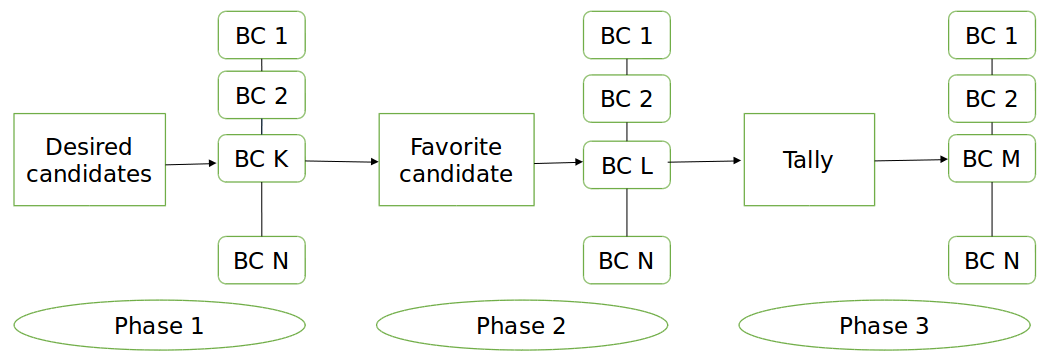
\includegraphics[width=80mm]{Flowdiagram.png}
	\caption{A visualization of the phases during the voting process. Voters select their desired candidates and save them to a blockchain. Then given the selected candidates, voters select their favorite candidate and save them to a blockchain. Then when every voter has voted, they tally the votes and save their tally along with their name to a blockchain. The sets of blockchains for each phase are disjoint.}
\end{figure}


\subsection{Phase One}
Phase one sets up the vote to ensure all voters are voting on the same thing. Each voter saves their desired candidates to a block and appends that block to the longest blockchain with the same desired candidates. If no blockchain exists then they create a blockchain. Given the assumption that each group of voters with an agreed upon group of candidates will append the same blockchain, the largest group of voters must have appended the longest blockchain. This ensures the largest group of voters with the same desired candidates will have their blockchain accepted by all peers. 

Multiple metrics for determining when to end phase one are relevant. We chose to end phase one when every voter appended the accepted blockchain. This was implemented by having each voter save a group of desired voters, which relates to the authentication feature as discussed in section 3.D.3, then comparing the voters who appended that blockchain with the desired voters. Other acceptable criteria for determining when to end phase one may be time based, waiting for a majority of desired voters to vote, or some hybrid of the two where the longer phase one lasts, the fewer the voters that need to be involved in phase one. 

\subsection{Phase Two}
Phase two allows the voters to vote on their favorite candidate given the desired candidates in the accepted blockchain from phase one. Each voter saves the candidate they are voting for to a block and appends that block to the longest blockchain. Blockchains appended in phase two are different blockchains than those appended in phase one. If no blockchain exists then they create a blockchain. During this phase, there aren't multiple blockchains due to varying contents but simply due to the curse of distributed systems; multiple voters may cast their votes in unison resulting in multiple blockchain forks appended from the same blockchain. Upon sharing these blockchains, a voter who has already voted may receive a longer blockchain which they have not casted their vote to. They must then cast their vote to this longer blockchain. At the end of phase two, the longest blockchain is the accepted blockchain.

The same metrics for determining when to end phase one hold for determining when to end phase two. 

\subsection{Phase Three}
Phase three allows the voters to tally the votes in the accepted phase two blockchain. Each voter will begin tallying the longest blockchain in their possession. If they acquire a longer blockchain during this process, they will restart with the longer blockchain. Upon completing their tally, each voter saves their tally along with their name to a block and appends that block to the longest blockchain with the same tally. They save their name to the block to ensure unauthorized voters don't cast tallies since a large enough group of unauthorized voters could cast fake tallies and ultimately alter the result. The multiple blockchains is made possible both by the curse of distributed systems and through varying contents; different tallies are appended to different blockchains. Same as during the first two phases, the longest blockchain is accepted and the contained tally of that blockchain is the official tally of the vote.

The metrics for determining when to end phase three are slightly different than those for determining when to end phases one and two. Since only a majority of votes are required for determining a selected candidate, phase three can end when the longest blockchain contains a tally from a majority of the voters. Otherwise, the same metrics apply as those from the first two phases. 

\subsection{Feature Support}
The description of the system as explained thus far is a bare bones implementation and does not include any of the features described in section 1. Thus far we have made assumptions such as no voter will vote more than once, unauthorized voters will not vote, no one will attempt to modify other voter's vote, along with many other naive assumptions. These features aim to ensure all attacks on the integrity of the voting system are blocked.

\subsubsection{Uniqueness}
In many democratic voting processes, a voter may only vote once, and their vote only counts for a single vote. In phase two, we can have every voter save their name, or some identifier, to their block. A voter voting repeatedly isn't viewed as multiple votes but simply changing their vote. This is ensured in phase three during the tally process where each voter will only count the last vote provided by each voter. 

\subsubsection{Authentication}
Many voting processes have restrictions on who can vote. To ensure only authorized voters may vote, during phase one, along with agreeing on the candidates, voters will also agree on the voters. Voters will only append their blocks to blockchains with the same desired voters as well as desired candidates. This will not affect phase two, but during phase three, voters will only count the votes of the voters in the accepted phase one blockchain.

\subsubsection{Integrity}
Once votes are cast, they shouldn't be modifiable by third parties. Votes are modifiable by the voter through simply recasting their vote, but to ensure third parties can't modify the blocks, some derivation of Proof-of-Work should be implemented. Proof-of-Work is essentially a puzzle which must be solved before a block can be appended to a blockchain. Proof-of-Work protocols are usually implemented such that multiple peers aid in appending a single block to a blockchain. So if more peers aid in appending the blockchain than modifying the blockchain, then the votes are protected from being modified by third parties. 

\subsubsection{Anonymity}
Voters may wish to be discrete regarding who or what they voted for. By simply not saving their name or any personal identifier to their block, this can be ensured. Unfortunately this would interfere with other features such as authentication so we attempt to solve this issue while still saving personal identifiers to the blocks. 

\subsubsection{Fairness}
If voters can determine the current trend of votes before the end of the voting period, it may influence their vote. To counter this, we wish for the votes to be kept secret until the voting period has expired. This can be accomplished through encryption. Each voter will encrypt their vote during phase two. During phase three, each voter will broadcast their key so each other voter can read and tally the votes. The difficulty with this is knowing which block each key belongs to. If the voters saved their name to the block then their name can be passed along with the key but this violates anonymity. If each block is assigned an unique identifier, then the identifier can be passed with the key but if someone can determine which voter transmitted the identifier then it still violates anonymity. Through transmitting a random subset of known keys and identifiers to the other voters, it will make it difficult for anyone to determine which voter casted which vote since it's unclear if the voter is passing their key and identifier or if they're simply relaying someone else's.

\subsubsection{Correctness}
It's a common ordeal that someone doesn't trust the tally was counted correctly and demands a recount. This assumes that a tally can be miscounted. Phase three is designed to ensure accuracy and honesty. Each voter tallies the votes and saves their tally to a blockchain with similar tallies. The longest blockchain all with the same tally is assumed to be correct. Since everyone has access to this tally, a false tally is unlikely to dominate all other tallies. 

\subsubsection{Robustness}
Simply by being a distributed system, this system is more fault tolerant than a centralized systems with few points of failure. The major weakness in this system is invalid blockchains don't dominate the valid blockchains. This is ensured through some derivation of Proof-of-Work which ensures malicious attackers are unlikely to modify the blockchain faster than the honest voters assuming less than a majority of those with access to the blockchains are malicious. 

\subsubsection{Verifiability}
Given most voting systems, it is unclear whether or not your vote counted. Phase three ensures all voters can determine their vote counted through the self-tally process. Each voter tallies the votes and during that process, assuming they voted, they'll tally their own vote. Unless they tally incorrectly, if their tally matches the accepted tally then their vote must have counted. 

\subsubsection{Coercion Freeness}
Voters could feasibly be coerced into voting for something or someone out of fear or temptation. Some of the previous features aim to minimize this coercion. Anonymity aims to alleviate fear out of others knowing who or what you voted for. Fairness aims to alleviate temptation into voting for something or someone they wouldn't have voted for had they not been given that information. Unfortunately there's potential for a third party standing over a voters shoulder as they vote. Voters could setup aliases or shortcuts for voting for a certain candidate ahead of time. This would allow the voter to essentially enter an encrypted vote even in the presence of a third party where as the third party would have no idea as to who or what the voter voted for. 

\section{Implementation}
The design as described in section 3 sound good in theory but it's always a different story when implementing and testing. We're in progress of implementing this system but we still have a ways to go.

A P2P network has been implemented. Since peers can't access a P2P network without prior knowledge of at least one peer, or broadcasting to the whole world, a server runs which stores the addresses of all known active peers. The server is launched with no known peers. The server's address is hard-coded into each of the peers so when the peer launches, it queries the server for known peers and saves their addresses. The peer routinely queries the server for any updates on known peers. The server also routinely queries the peer to ensure the peer is still active. If the peer doesn't respond to the server, the server assumes the peer is no longer active. When the peers have addresses with other peers, each peer will routinely request all blockchains from every other known peer. Upon request, the peer would gather all their blockchains and transmit them to the peer who requested. Upon receipt, the peer will overwrite all blockchains with the same identifier which are shorter. This process runs in the background while the voting process is taking place.

The voting process unfortunately doesn't contain all the features described above yet but it's a work in progress. All 3 phases function individually don't smoothly transition between phases without user intervention. The desired voters and desired candidates are hard-coded and not input by the user. Upon launch, the user is prompted for their name. The program then automatically creates a block with the desired voters and desired candidates and either appends the largest known blockchain with similar candidates and voters or it creates a new blockchain. This process blocks in phase one until all desired voters have agreed on a single set of desired voters and desired candidates then the program stops with saved blockchains. The user then manually starts phase two. The program prompts the user for a candidate, searches for the longest known blockchain and appends a block with the candidate. The program then exits. The user must manually start phase three. This program then searches for the longest phase two blockchain and tallies the votes then saves the tally to the longest blockchain with the same tally.
\footnote{https://github.com/shamprasad/teamEvoting}

\section{Evaluation}
The P2P network is functional but inefficient. The peer queries the server and the server queries the peer which is redundant. The same result can be achieved by the peer requesting peers from the server which can count as a check-in from the peer to the server. When blockchains are transferred between peers, every blockchain is transferred which is unnecessary. Given large polls, many older forks may exist which are no longer relevant. Also, during phases one and three, if the contents of the blockchain don't reflect the voter's block contents, then those blockchains will never be appended anyway. This process can be streamlined to only transfer the sending peer's longest blockchain and the longest blockchain with content equivalent to receiving peer's block content. 

The voting system is also fully functional but the most obvious downfall is the need for the user to manually start each phase. Only phase one transitions smoothly but the metric for determining if phases two and three have not been implemented yet so the program simply exits after a appending the voter's block. Fortunately, some of the features have been implemented, although in a fashion which may affect other features when implemented in the future. Authentication is partly achieved in phase one with the voters agreeing on a set of authorized voters. This has yet to be extended to phase three where the voter's ensure only authorized voters are voting. Correctness is implemented in phase three. By having the voters tally the votes, they can agree on a tally and the tally is likely the correct tally. This assumes that a majority of those tallying the votes are not malicious and possess the accepted phase two blockchain. Verifiability is implemented in phase three by having the voters tally the votes. If the accepted tally is equivalent to a voter's tally, then that voter's vote likely counted unless the voter miscounted or doesn't possess the accepted blockchain. 

\section{Future Work}
Goals for the P2P network involve optimizing data transfer efficiency. The server need not query each peer since each peer already queries the server. Currently every blockchain is transferred, even dated forks. A heuristic should be used to decide which blockchains need to be transferred. A simple heuristic includes only transferring the largest blockchain and the largest blockchain containing content related to the requesting peer's block content. If the requester already possesses those blockchains, then no blockchains shall be transferred. Also blockchains are passed as a single message. As blockchains grow, this will become infeasible. The blockchains should be partitioned so that they can be passed as a series of smaller chunks. Also, it may be feasible to request chunks of the same blockchain from separate peers such that it transfers more quickly. This may be a necessity given really large blockchains. To increase robustness, each peer can save a database of previously connected peers so if there is any issue with contacting the server, the peer could query those saved peers and hopefully they're active. 

Goals for the voting system include implementing the metric for determining when a phase has finished. This will allow smoothly transitioning between phases without user intervention. Modify phase three to ensure only valid voters may vote and only the last vote counts. Design, implement, and test some derivation of Proof-of-Work to ensure no one can control a blockchain and no one can modify votes. Implement a encryption technique for encrypting a voter's vote then passing the key along with a block identifier to their peers upon entering phase three so the vote can be tallied. Implement an algorithm to randomly pass a subset of known keys and block ids to ensure the owner of the key and block id are kept anonymous. Implement the option for voting candidate aliases or shortcuts.

% An example of a floating figure using the graphicx package.
% Note that \label must occur AFTER (or within) \caption.
% For figures, \caption should occur after the \includegraphics.
% Note that IEEEtran v1.7 and later has special internal code that
% is designed to preserve the operation of \label within \caption
% even when the captionsoff option is in effect. However, because
% of issues like this, it may be the safest practice to put all your
% \label just after \caption rather than within \caption{}.
%
% Reminder: the "draftcls" or "draftclsnofoot", not "draft", class
% option should be used if it is desired that the figures are to be
% displayed while in draft mode.
%
%\begin{figure}[!t]
%\centering
%\includegraphics[width=2.5in]{myfigure}
% where an .eps filename suffix will be assumed under latex, 
% and a .pdf suffix will be assumed for pdflatex; or what has been declared
% via \DeclareGraphicsExtensions.
%\caption{Simulation results for the network.}
%\label{fig_sim}
%\end{figure}

% Note that IEEE typically puts floats only at the top, even when this
% results in a large percentage of a column being occupied by floats.


% An example of a double column floating figure using two subfigures.
% (The subfig.sty package must be loaded for this to work.)
% The subfigure \label commands are set within each subfloat command,
% and the \label for the overall figure must come after \caption.
% \hfil is used as a separator to get equal spacing.
% Watch out that the combined width of all the subfigures on a 
% line do not exceed the text width or a line break will occur.
%
%\begin{figure*}[!t]
%\centering
%\subfloat[Case I]{\includegraphics[width=2.5in]{box}%
%\label{fig_first_case}}
%\hfil
%\subfloat[Case II]{\includegraphics[width=2.5in]{box}%
%\label{fig_second_case}}
%\caption{Simulation results for the network.}
%\label{fig_sim}
%\end{figure*}
%
% Note that often IEEE papers with subfigures do not employ subfigure
% captions (using the optional argument to \subfloat[]), but instead will
% reference/describe all of them (a), (b), etc., within the main caption.
% Be aware that for subfig.sty to generate the (a), (b), etc., subfigure
% labels, the optional argument to \subfloat must be present. If a
% subcaption is not desired, just leave its contents blank,
% e.g., \subfloat[].


% An example of a floating table. Note that, for IEEE style tables, the
% \caption command should come BEFORE the table and, given that table
% captions serve much like titles, are usually capitalized except for words
% such as a, an, and, as, at, but, by, for, in, nor, of, on, or, the, to
% and up, which are usually not capitalized unless they are the first or
% last word of the caption. Table text will default to \footnotesize as
% IEEE normally uses this smaller font for tables.
% The \label must come after \caption as always.
%
%\begin{table}[!t]
%% increase table row spacing, adjust to taste
%\renewcommand{\arraystretch}{1.3}
% if using array.sty, it might be a good idea to tweak the value of
% \extrarowheight as needed to properly center the text within the cells
%\caption{An Example of a Table}
%\label{table_example}
%\centering
%% Some packages, such as MDW tools, offer better commands for making tables
%% than the plain LaTeX2e tabular which is used here.
%\begin{tabular}{|c||c|}
%\hline
%One & Two\\
%\hline
%Three & Four\\
%\hline
%\end{tabular}
%\end{table}


% Note that the IEEE does not put floats in the very first column
% - or typically anywhere on the first page for that matter. Also,
% in-text middle ("here") positioning is typically not used, but it
% is allowed and encouraged for Computer Society conferences (but
% not Computer Society journals). Most IEEE journals/conferences use
% top floats exclusively. 
% Note that, LaTeX2e, unlike IEEE journals/conferences, places
% footnotes above bottom floats. This can be corrected via the
% \fnbelowfloat command of the stfloats package.



% conference papers do not normally have an appendix


% use section* for acknowledgment


% trigger a \newpage just before the given reference
% number - used to balance the columns on the last page
% adjust value as needed - may need to be readjusted if
% the document is modified later
%\IEEEtriggeratref{8}
% The "triggered" command can be changed if desired:
%\IEEEtriggercmd{\enlargethispage{-5in}}

% references section

% can use a bibliography generated by BibTeX as a .bbl file
% BibTeX documentation can be easily obtained at:
% http://www.ctan.org/tex-archive/biblio/bibtex/contrib/doc/
% The IEEEtran BibTeX style support page is at:
% http://www.michaelshell.org/tex/ieeetran/bibtex/
%\bibliographystyle{IEEEtran}
% argument is your BibTeX string definitions and bibliography database(s)
%\bibliography{IEEEabrv,../bib/paper}
%
% <OR> manually copy in the resultant .bbl file
% set second argument of \begin to the number of references
% (used to reserve space for the reference number labels box)
\begin{thebibliography}{1}

\bibitem{Nakamoto}
S.~Nakamoto, \emph{Bitcoin: A Peer-to-Peer Electronic Cash System}, 2008.
\bibitem{Followmyvote}
"The Online Voting Platform of the Future - Follow My Vite", \emph{Follow My Vote}, 2018. [Online]. Available: https://followmyvote.com/. [Accessed: 06-Apr-2018].
\bibitem{Liu}
Y.~Liu and Q.~Wang, \emph{An E-voting Protocol Based on Blockchain}, 2017.
\bibitem{Unchain}
"unchain.voting", \emph{Unchain.voting}, 2018. [Online]. Available http:\\www.unchain.voting/. [Accessed: 07-Apr-2018].
\bibitem{Publicvotes}
"PublicVotes: Ethereum-based Voting Application - Dominik Schiener - Medium", \emph{Medium}, 2018. [Online]. Available: https://medium.com/@DomSchiener/publicvotes-ethereum-based-voting-application-3b691488b926. [Accessed: 07-Apr-2018].

\end{thebibliography}




% that's all folks
\end{document}